\documentclass[prc]{revtex4}
\usepackage[dvips]{graphicx}
\usepackage{mathrsfs}
\usepackage{amsfonts}
\usepackage{lscape}

\usepackage{epic,eepic}
\usepackage{amsmath}
\usepackage{amssymb}
\usepackage[dvips]{epsfig}
\usepackage[T1]{fontenc}
\usepackage{hyperref}
\usepackage{bezier}
\usepackage{pstricks}
\usepackage{dcolumn}% Align table columns on decimal point
\usepackage{bm}% bold math
%\usepackage{braket}
\usepackage[dvips]{graphicx}
\usepackage{pst-plot}

\newcommand{\One}{\hat{\mathbf{1}}}
\newcommand{\eff}{\text{eff}}
\newcommand{\Heff}{\hat{H}_\text{eff}}
\newcommand{\Veff}{\hat{V}_\text{eff}}
\newcommand{\braket}[1]{\langle#1\rangle}
\newcommand{\Span}{\operatorname{sp}}
\newcommand{\tr}{\operatorname{trace}}
\newcommand{\diag}{\operatorname{diag}}
\newcommand{\bra}[1]{\left\langle #1 \right|}
\newcommand{\ket}[1]{\left| #1 \right\rangle}
\newcommand{\element}[3]
    {\bra{#1}#2\ket{#3}}

\newcommand{\normord}[1]{
    \left\{#1\right\}
}

\usepackage{amsmath}
\begin{document}
\title{Exercises FYS4480, week 45, November 7-11, 2022}

%\author{}
\maketitle

\subsection*{Exercise 1}

We consider a one-particle system with the following Hamiltonian
$H=H_{0}+H_{1}$ where
\[
H_{0}=\sum_{i=1,2}\varepsilon_{i}a_{i}^{\dagger}a_{i}
\]
\[
H_{1}=\lambda\sum_{i\neq j=1,2}a_{i}^{\dagger}a_{j}
\]
\begin{enumerate}
\item[a)] Find the ground state energy to third order in perturbation theory
using both Brillouin-Wigner and Rayleigh-Sch\"{o}dinger 
perturbation theory.
\item[b)] Write down the corresponding diagrams in the particle picture (using the true vacuum).
\item[c)] Find the exact energy and expand the exact results in terms of the
parameter $\lambda$ and compare with the results obtained with the above two
expansions. Discuss the eventual differences.
\item[d)] Rewrite the unperturbed ground state in 
the particle-hole representation
\[
\ket{c}=\ket{\Phi_{1}}=a_{1}^{\dagger}\ket{0},
\]
and write down the corresponding diagrams
\item[e)] To fourth order in perturbation theory we have unlinked diagrams.
Give examples of these and show how they can be cancelled.
\end{enumerate}

\subsection*{Exercise 2, time-ordered product}

Show that
\[
{\displaystyle\int_{t'}^{t}}dt_{1}{\displaystyle\int_{t'}
^{t_{1}}}dt_{2}H_{1}(t_{1})H_{1}(t_{2})=
\frac{1}{2}{\displaystyle\int_{t'}^{t}dt_{1}}{\displaystyle
\int_{t'}^{t}}dt_{2}T\left[H_{1}(t_{1})H_{1}(t_{2})\right]
\]
{\underline Hint:} Use the definition of $T$ in order to distinguish between
$t_{1}>t_{2}$ and $t_{1}<t_{2}$;
\[
{\displaystyle\int_{t'}^{t}}dt_{1}{\displaystyle\int_{t'}^{t}}
dt_{2}T\left[H_{1}(t_{1})H_{1}(t_{2})\right]
={\displaystyle\int_{t'}^{t}}dt_{1}\left\{{\displaystyle
\int_{t'}^{t_{1}}}dt_{2}H_{1}(t_{1})H_{1}(t_{2})+{\displaystyle
\int^{t}_{t_{1}}}dt_{2}H_{1}(t_{2})H_{1}(t_{1})
\right\}
\]
Show that the last term on the right-hand side equals the first term
(change the order of the integrations and thereafter integration variables).
The area of integration for the first term is shown in the figure below.
\begin{figure}[hbtp]
\includegraphics[width=.4\textwidth]{timeordering.ps}
\end{figure}




\end{document}
